
Each server in the mix-net perform the same actions during execution.

\begin{enumerate}
\item It is given the list of ciphertexts from the previous server.
\item It reencrypts these ciphertexts with its private key.
\item It randomly shuffles the list of ciphertexts.
\item It passes the reencrypted and shuffled list of ciphertexts to the next server.
\end{enumerate}

During these steps a zero-knowledge proof is produced which can prove that the server indeed did output a list of shuffled and reencrypted ciphertexts without tampering with the ciphertexts.

\begin{center}
  \makebox[\textwidth]{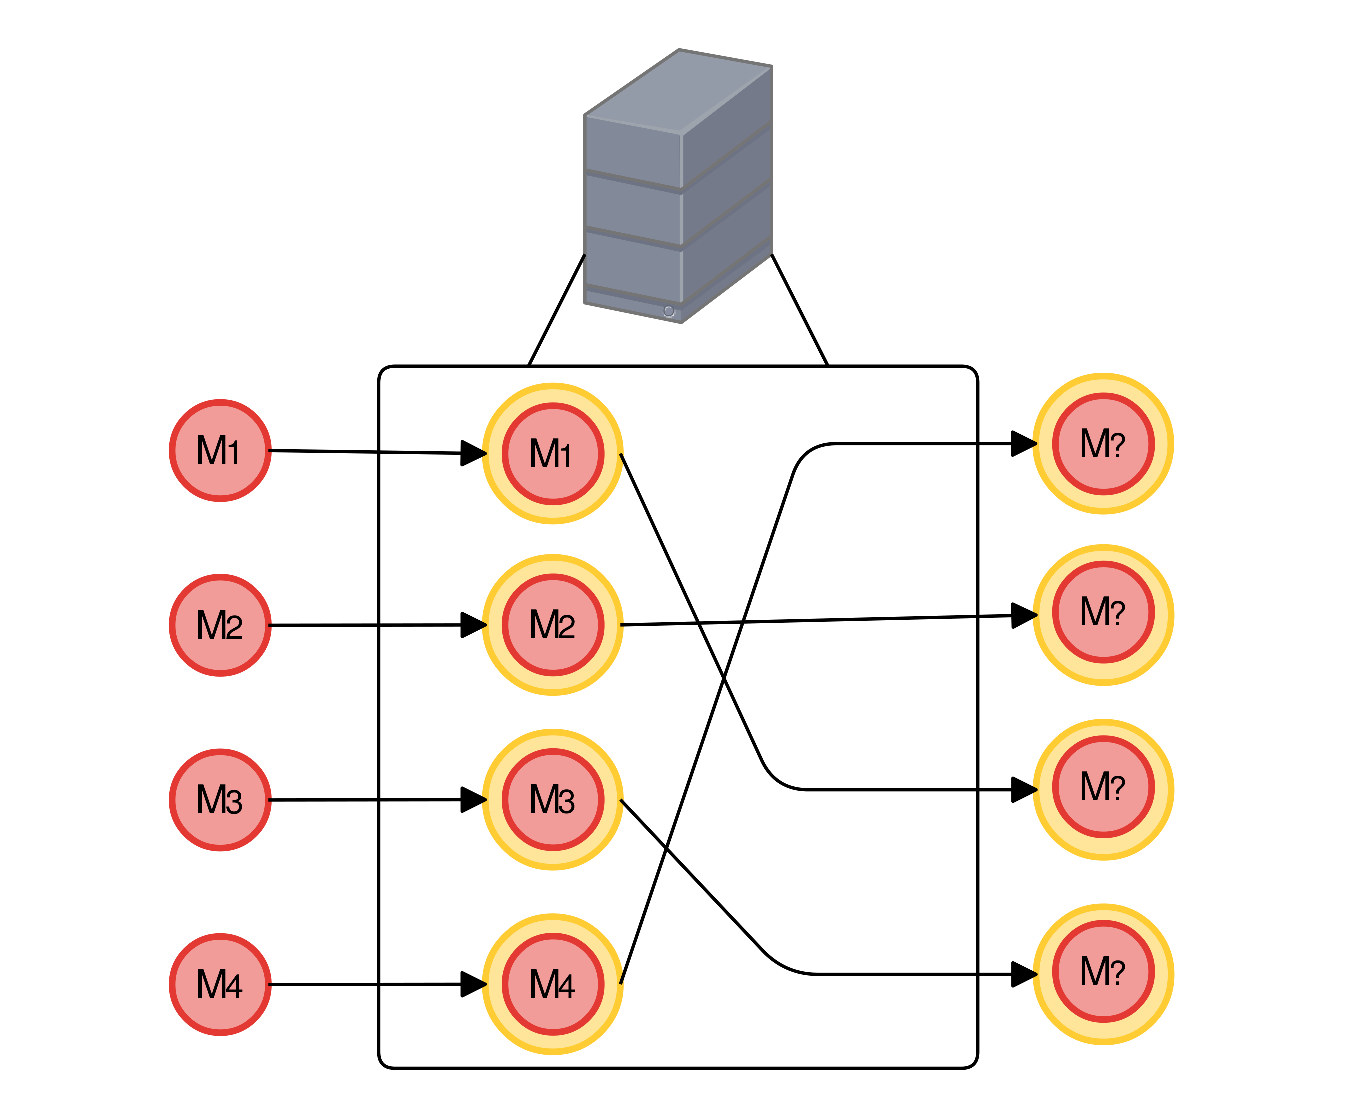
\includegraphics[width=0.7\textwidth]{../presentation/images/mix4.pdf}}
\end{center}
